\section{Experimental Results}

\begin{table}
\begin{center}
\begin{tabular}{>{\bfseries}ll}
Manufacturer         & Intel Corp.\\
CPU Name             & Core i7-3520M\\
L1-Cache             & 32 KB\\
L2-Cache             & 256 KB\\
L3-Cache             & 4 MB\\
CPU-core frequency   & 2901 MHz\\
Scalar FP-Add Cycles/issue  & 1\\
Vect. FP-Add Cycles/issue (SSE) & 2\\
Vect. FP-Add Cycles/issue (AVX) & 4\\
\end{tabular}
\end{center}
\caption{Processor details.}
\label{tab:processor}
\end{table}

This section assesses the performance increase in the algorithm based on
the methods described in the previous section. The test machine and
software tools used are presented.

\mypar{Measurement Setup}
Measurements were performed on a Lenovo ThinkPad T430s with 8 GiB RAM and
the processor shown in \autoref{tab:processor}. The operating system was
Kubuntu 14.04 64-bit. The compiler used was the GNU C Compiler 4.8.2 with
the flags:
\begin{verbatim}
-O3 -m64 -march=corei7-avx -mavx
  -fno-tree-vectorize
\end{verbatim}

Peak performance is equal to the floating point additions cycles/issue of
the processor, see \autoref{tab:processor}, since our algorithm does not
perform any other floating point operations. That is, 1 fl/c for scalar
code, 2 fl/c for SSE and 4 fl/c for AVX code.
To asses the performance, libperfmon
4\footnote{\url{http://perfmon2.sourceforge.net/}} was used to measure the
number of cycles. The results were obtained by averaging over 10
consecutive executions for a given problem size.
To obtain the measurement data for the roofline-plots, perfplot was used,
together with libpcm 2.6.

There is a crucial difference between the performance plots and the roofline
plots: For the latter, all floating point operations were counted, including
comparisons, whereas for the former, the number of additions from the cost
analysis was used as a basis.

We used randomized input data for our computation. To have reproducible
results, the seed was fixed.

\begin{figure}[htb]\centering
  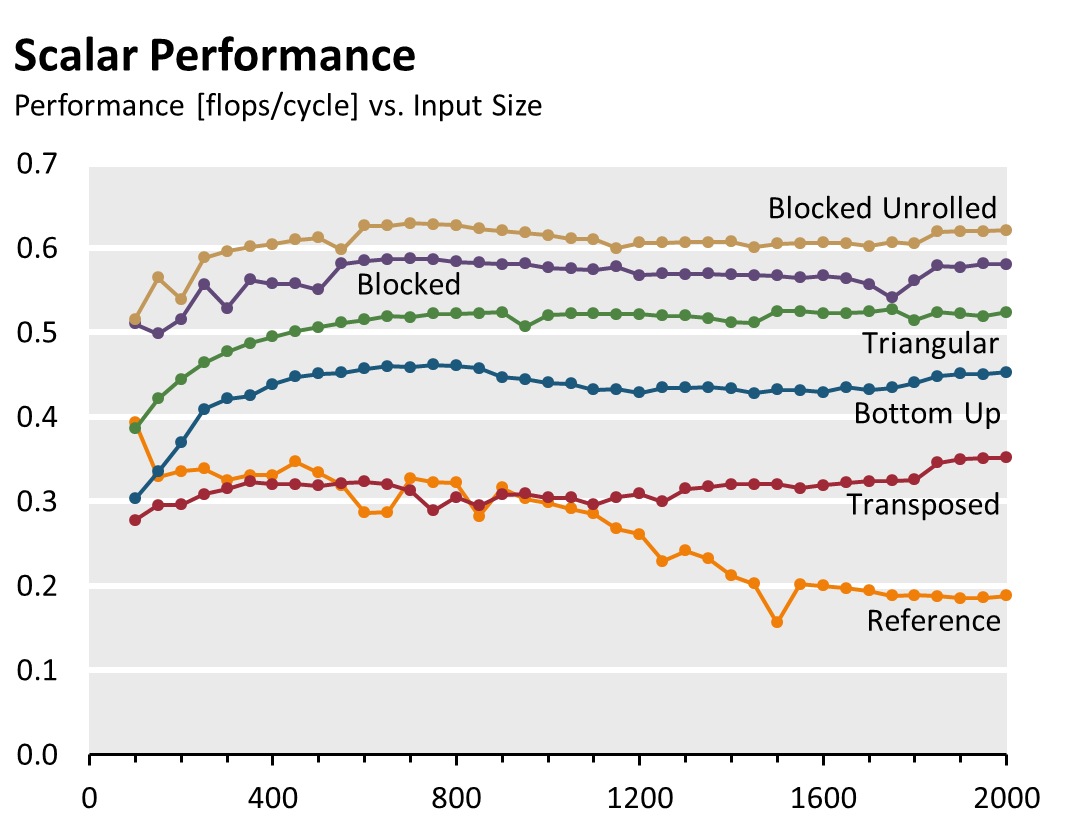
\includegraphics[width=\linewidth]{plot_data/scalar_performance.png}
  \caption{Performance of the scalar implementations.}
  \label{fig:perf-scalar}
\end{figure}
\mypar{Scalar Performance}
\autoref{fig:perf-scalar} shows the performance of the different scalar
implementations. Peak performance lies at 1 fl/c. The reference
implementation has a performance of 0.2 fl/c for large input sizes. Using
the \emph{transposed} approach improving spatial locality, we can already
see stable performance for large input sizes that do no longer fit the last
level cache. We can again see the expected performance boost when changing
the access pattern of the table to \emph{bottom-up}, thanks to further
improved spatial locality. With a performance of about 4.5 fl/c, this
corresponds to a performance gain of more than 2x to the baseline. Changing
to the triangular memory layout improves performance to up to 0.5 fl/c. We
assume this is due to the increased performance of the CPU prefetcher.
However, we were not able to verify this. The \emph{blocking} approach,
based on the squared memory layout, gives another performance boost due to
increased reuse in the CPU registers and fewer memory write-backs. The
final scalar performance of our implementation lies at 62\% peak
performance which is equivalent to a performance gain of roughly 3x.

\begin{figure}[htb]\centering
  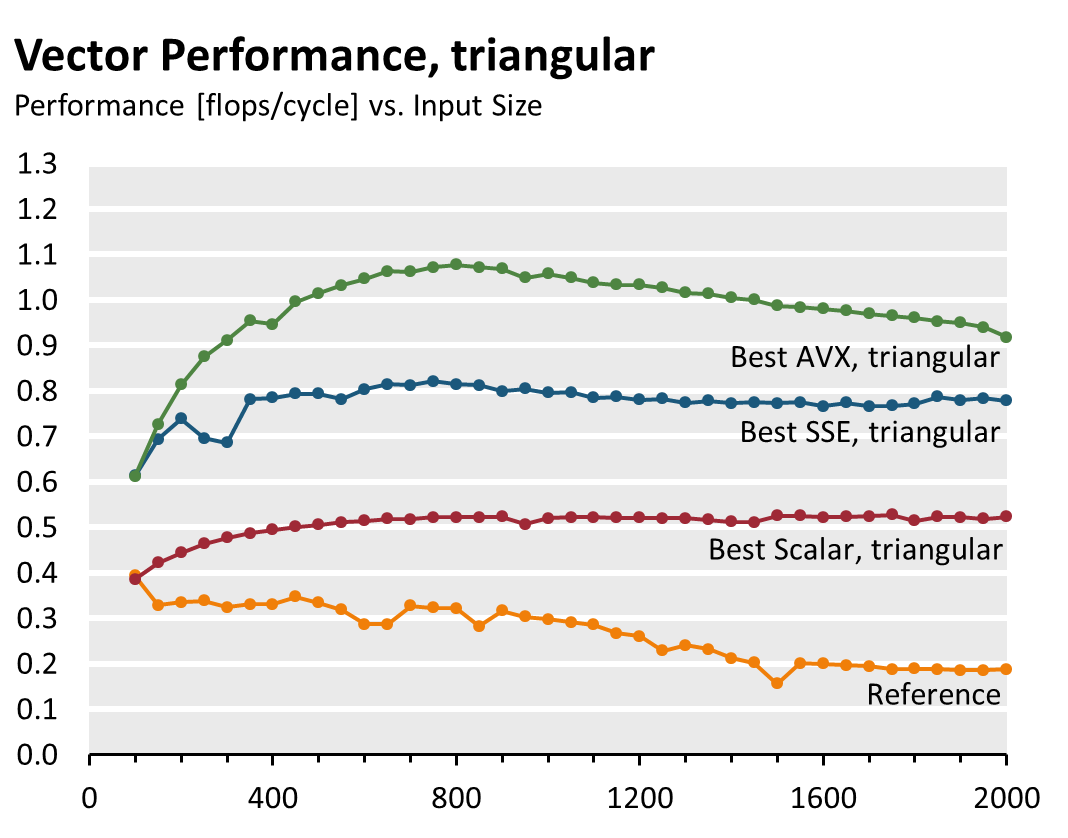
\includegraphics[width=\linewidth]{plot_data/triangular_vector_performance.png}
  \caption{Vectorized Performance based on \emph{Triangle}.}
  \label{fig:perf-triangular}
\end{figure}
\mypar{Vectorized Performance, triangular}
\autoref{fig:perf-triangular} shows the performance of our SSE and AVX
vector code based on the \emph{Triangle} scalar code. With 0.8 fl/c
performance for the SSE code, the speedup through vectorization lies at
1.6x below the theoretical maximum of 2x. From SSE to AVX, the speedup lies
at 1.2x compared to the expected 2x. Overall, the speedup from the baseline
lies at 4.6x.

\begin{figure}[htb]\centering
  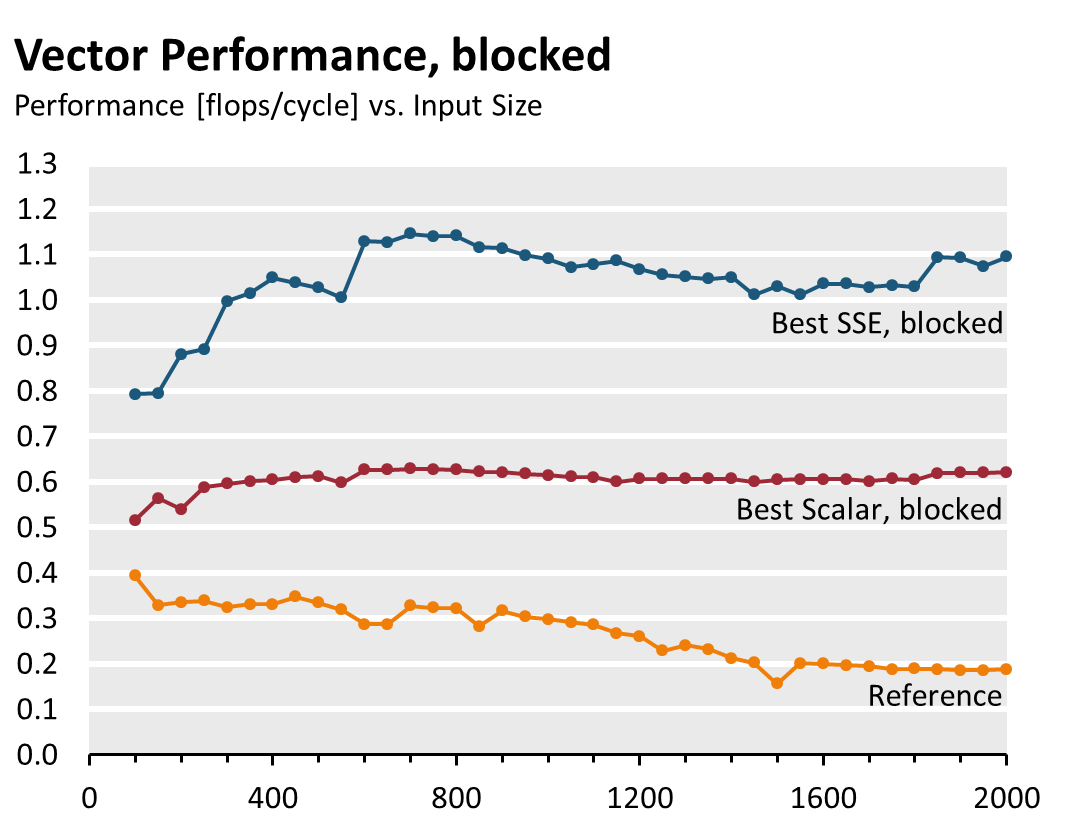
\includegraphics[width=\linewidth]{plot_data/blocked_vector_performance.png}
  \caption{Vectorization based on \emph{Blocking}.}
  \label{fig:perf-blocked}
\end{figure}
\mypar{Vectorized Performance, blocked}
\autoref{fig:perf-blocked} shows the performance of our SSE vector code
based on the \emph{Blocked} approach. The AVX variant performance worse and
is thus omitted. Having a performance of about 1.1 fl/c, the SSE code
yields a 1.8x speedup compared to the best scalar code and a 5.5x speedup
to the baseline implementation. Note that the blocking SSE code performs
better than the triangular AVX code.

\begin{figure}[htb]\centering
  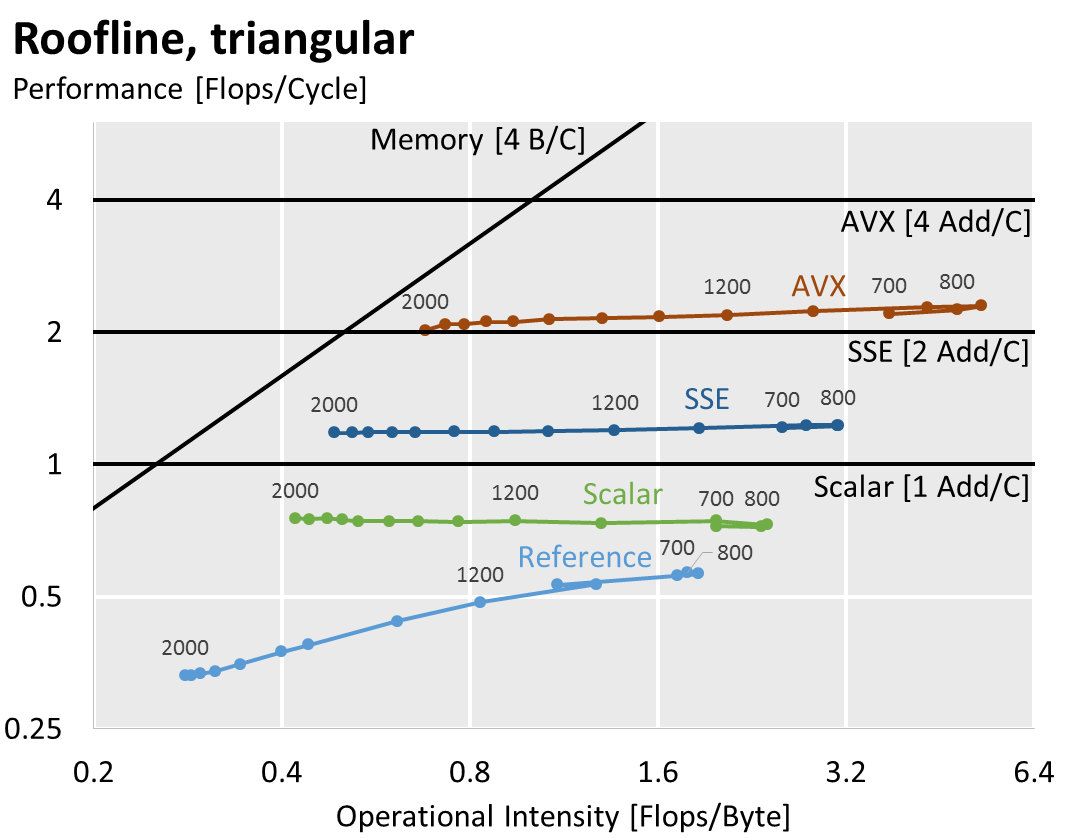
\includegraphics[width=\linewidth]{roofline-data/roofline_triangular.png}
  \caption{Roofline Plot based on \emph{Triangle}.}
  \label{fig:roofline-triangular}
\end{figure}
\begin{figure}[htb]\centering
  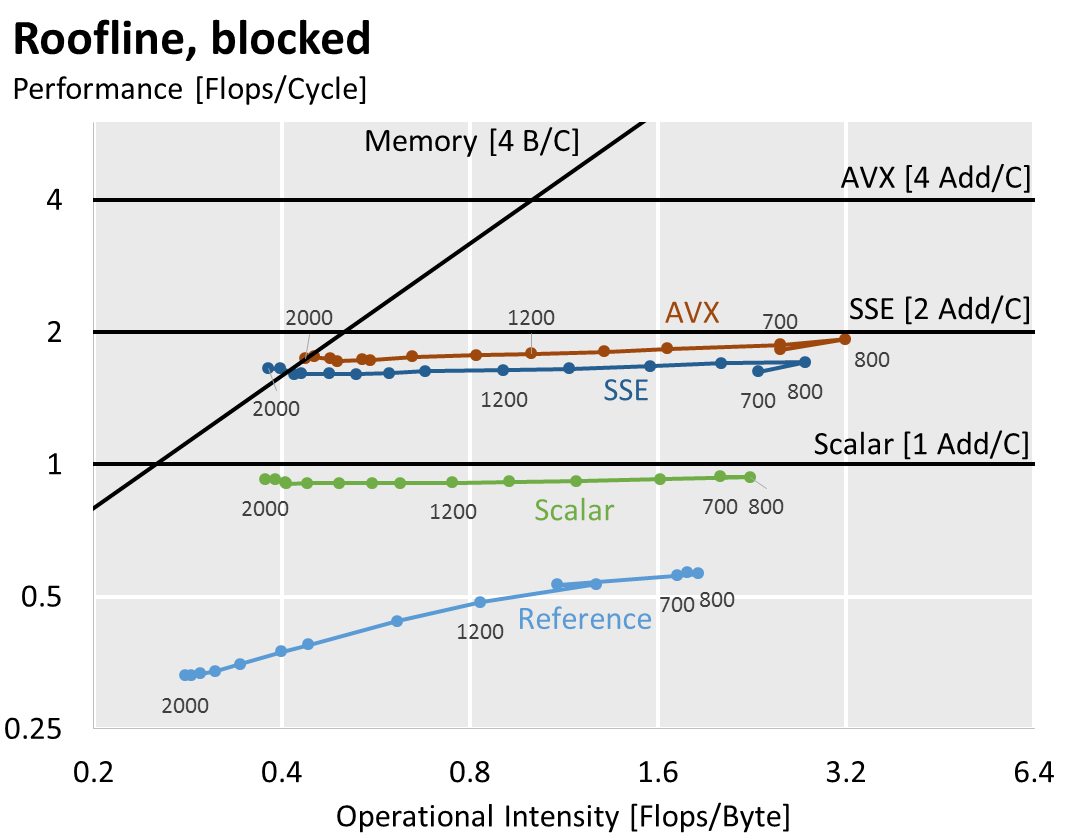
\includegraphics[width=\linewidth]{roofline-data/roofline_blocked.png}
  \caption{Roofline Plot based on \emph{Blocked}.}
  \label{fig:roofline-blocked}
\end{figure}
\mypar{Roofline Analysis}
\autoref{fig:roofline-triangular} and \autoref{fig:roofline-blocked} show
the roofline plots of our respective solutions. Note that for the roofline
plots, libpcm was used to measure all floating point operations including
comparisions. Thus, performance numbers are different than in the
performance plots. We can see in \autoref{fig:roofline-blocked}, scalar
performance is almost at the peak of 1 fl/c. Also, the SSE code comes close
to optimal. In contrast to the performance plots using our theoretical flop
count, here the AVX variant performs slightly better than the SSE one. The
blocked scalar and SSE versions are the fastest for their category. For the
\emph{Triangle} case in \autoref{fig:roofline-triangular}, we have the best
overall performance with the AVX variant yielding around 2 fl/c. This
corresponds to an overall speedup achieved of roughly 6x.
